

我们已经讨论了软件代码的文档化和图形化,但在大型项目中,可能还需要文档化和可视化CMake代码。CMake目标之间的关系可能很复杂,这可能使跟踪所有依赖关系变得困难。CMake可以通过提供一个显示目标之间所有依赖关系的图表来帮助解决这个问题。通过cmake -{}-graphviz=my-project.dot /path/to/build/dir,CMake将用dot创建包含目标如何相互依赖的文件。

DOT语言是一种用于图形的描述语言,可以由许多程序进行解释,其中最著名的是免费的Graphviz。DOT文件可以使用Graphviz中的DOT命令行实用程序转换为图像,甚至可移植文档格式(PDF)文件:dot -Tpng filename.dot -o out.png。

为本章的示例项目运行这些命令将产生类似如下的输出:

\begin{center}
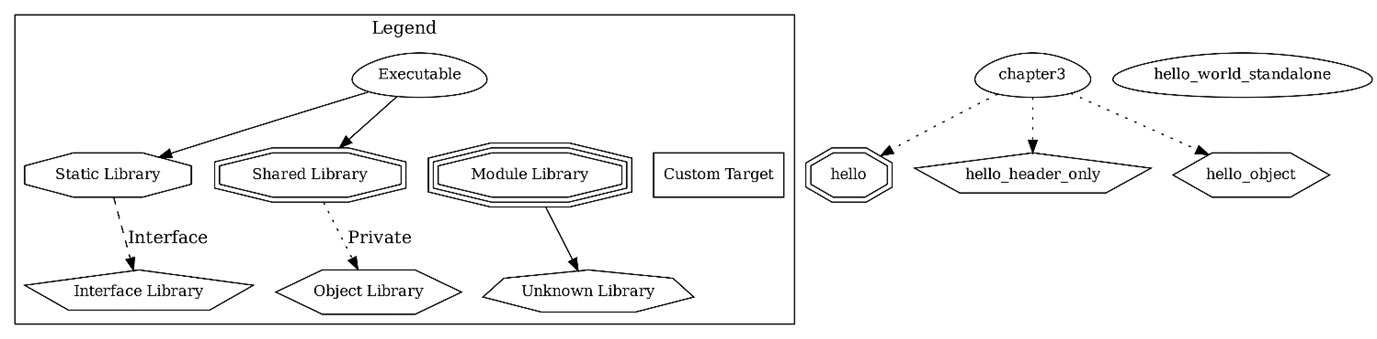
\includegraphics[width=0.9\textwidth]{content/2/chapter6/images/7.jpg}\\
图6.7 用DOT语言可视化的第3章的项目结构
\end{center}

行为和选项可以通过CMakeGraphVizOptions中提供的变量来控制。创建DOT图时,CMake将查找一个名为CMakeGraphVizOptions的文件。若在PROJECT\_SOURCE\_DIR和PROJECT\_BINARY\_DIR目录中找到,将使用其中提供的值。配置文件的例子:

\begin{lstlisting}[style=styleCMake]
set(GRAPHVIZ_GRAPH_NAME "CMake Best Practices")
set(GRAPHVIZ_GENERATE_PER_TARGET FALSE)
set(GRAPHVIZ_GENERATE_DEPENDERS FALSE)
\end{lstlisting}

默认情况下,CMake为所有目标创建依赖关系图。将GRAPHVIZ\_GENERATE\_PER\_TARGET和GRAPHVIZ\_GENERATE\_DEPENDERS设置为FALSE将减少生成的文件数量。可以在CMake文档\url{https://cmake.org/cmake/help/latest/module/CMakeGraphVizOptions.html}中找到完整的选项集。

















